% Auriga theme
% https://github.com/anishathalye/auriga

\documentclass[14pt,aspectratio=169]{beamer}
\usepackage{pgfpages}
\usepackage{fancyvrb}
\usepackage{booktabs,dcolumn}
\usepackage{tikz}
\usetikzlibrary{arrows.meta, positioning, quotes}
\usepackage{pgfplots}

% \ifnotes
% \setbeamertemplate{note page}[plain]
% \setbeameroption{show notes on second screen=right}
% \fi

\usetheme{auriga}
\usecolortheme{auriga}

% define some colors for a consistent theme across slides
\definecolor{red}{RGB}{181, 23, 0}
\definecolor{blue}{RGB}{0, 118, 186}
\definecolor{gray}{RGB}{146, 146, 146}

\title{Historia Económica Argentina}

\author{\underline{Sebastián Freille} \inst{1}}

\institute[shortinst]{\inst{1} IEF-UNC \\ UCC}
\date{}

\AtBeginSection[]{
    \begin{frame}
    \vfill
    \centering
    \begin{beamercolorbox}[sep=8pt,center,shadow=true,rounded=true]{title}
        \usebeamerfont{title}\insertsectionhead\par%
    \end{beamercolorbox}
    \vfill
    \end{frame}
}



\AtBeginSubsection[]{
    \begin{frame}
    \vfill
    \centering
    \begin{beamercolorbox}[sep=6pt,center,shadow=true,rounded=true]{title}
        \usebeamerfont{title}\insertsubsectionhead\par%
    \end{beamercolorbox}
    \vfill
    \end{frame}
}


\AtBeginSubsubsection[]{
    \begin{frame}
    \vfill
    \centering
    \begin{beamercolorbox}[sep=4pt,center,shadow=true,rounded=true]{title}
        \usebeamerfont{title}\insertsubsubsectionhead\par%
    \end{beamercolorbox}
    \vfill
    \end{frame}
}


\begin{document}

{
  % rather than use the frame options [noframenumbering,plain], we make the
  % color match, so that the indicated page numbers match PDF page numbers
  \setbeamercolor{page number in head/foot}{fg=background canvas.bg}
  \begin{frame}
    \titlepage
  \end{frame}
}

  
  \section{Capítulo 2. Los años entre las dos guerras (1914-1945)}


  \subsection{Los años veinte, 1919-1928}


 \begin{frame}\frametitle{Los años veinte, 1919-1928}
    \begin{itemize}\itemsep 10pt
      \item Apenas terminada la guerra toda la demanda reprimida
        afloró y esto generó un combo de expansión (boom) con
        inflación: la guerra había destruido parte del capital e
        infraestructura y esto afectó la oferta. Además, PF y PM
        expansivas estimularon aún más la demanda
        \item El boom fue de corta duración. Pronto los países
          empezaron a subir la tasa de interés. Primero EEUU, a lo que
          siguió nuevos aumentos de Francia y Gran Bretaña para evitar
          nuevas salidas de reservas
                 \end{itemize}
      \end{frame}
  


 \begin{frame}\frametitle{Los años veinte, 1919-1928 (cont.)}
   \begin{block}{Cambio de régimen}
     Este período definió una transición crítica en la
       historia económica
Argentina. Casi todos los historiadores coinciden en que es durante
este periodo que se opera un \textit{cambio de régimen}. Este cambio
es mejor expresado por el gradual movimiento desde la convergencia y
prosperidad relativa hacia una divergencia y atraso relativo. Todas
las historias destacan este periodo como el inicio de este régimen de
cambio --algunos incluso definen al año 1929 como el punto de quiebre
decisivo. 
     \end{block}
      \end{frame}


\begin{frame}\frametitle{Los años veinte, 1919-1928 (cont.)}
    \begin{itemize}\itemsep 10pt
      \item Es importante notar algunas diferencias importantes en la
        performance tanto del \textbf{sistema monetario} y del
        \textbf{sistema financiero} en Argentina en este periodo
        inter-guerras
        \item El sistema monetario argentino exhibió una continuidad
          bastante importante entre 1890 y 1935 bajo el comando de la
          CdC y su apego a reglas estrictas de emisión
          \item El sistema financiero local sin embargo, luego de
            haber sido destruido en 1890, se habia expandido hasta
            incluir mercados bancarios, acciones y deuda
       \end{itemize}
      \end{frame}
  

\begin{frame}\frametitle{Los años veinte, 1919-1928 (cont.)}
    \begin{itemize}\itemsep 10pt
      \item Dos cuestiones fundamentales en relación a la extensión y
        solidez de este sistema finaciero son relevantes:
        \begin{itemize}\itemsep 10pt \medskip
        \item ¿Cuán importante era el desarrollo del sistema
          financiero en Argentina comparado con el periodo previo y
          contra otros países? $\longrightarrow$ tamaño del mercado y
          perspectivas de ahorro, inversión y crecimiento a LP
          \item ¿Cuáles eran las fuentes de inestabilidad
            macroeconomica originadas por shocks financieros en este
            sistema? $\longrightarrow$ fragilidad inherente del sistema
          \end{itemize}
       \end{itemize}
      \end{frame}

      


\begin{frame}\frametitle{Los años veinte, 1919-1928 (cont.)}
    \begin{itemize}\itemsep 10pt
      \item En los años 20s Argentina tenía un grado importante de
        desarrollo financiero pero tal vez no lo que se hubiera
        deseado.
        \item Por ejemplo, cuentas de ahorro crecieron de del 8\% al
          22\% entre 1913-14 y 1928-29 y el grado de monetización
          pasó de 46\% al 55\% en este mismo período
          \item Pero el mercado de renta variable era casi
            inexistente $\longrightarrow$ compañías dependian de
            banca comercial (CP) y de utilidades propias (LP) 
       \end{itemize}
      \end{frame}
  
      

\begin{frame}\frametitle{Los años veinte, 1919-1928 (cont.)}
    \begin{itemize}\itemsep 10pt
      \item El sistema bancario dependía fuertemente de una
        entidad --BNA tenía 2/5 todos los activos bancarios. En
        ausencia de Banco Central tenía un rol cuasi-público.
        \item Es importante notar que la mitad del stock de capital
          argentino en 1913 era de propiedad extranjera (en su gran
          mayoría británico)
          \item ¿Por qué era Argentina tan dependiente del capital
            extranjero entre 1890 y 1914? Dos explicaciones
            potenciales: 1) desarrollo ``parado'' del sistema
            financiero argentino impedía movilización de fondos; 2)
            peso del crecimiento demográfico 
       \end{itemize}
      \end{frame}
  


\begin{frame}\frametitle{Los años veinte, 1919-1928 (cont.)}
    \begin{itemize}\itemsep 10pt
      \item Ante la presencia de cualquiera (o ambas) de estas
        características, es facil ver como un corte abrupto de
        entradas de capital causa problemas en la inversión y el
        crecimiento
        \item Ambas características son mas bien estructurales y de
          largo plazo $\longrightarrow$ modificarlas lleva tiempo. Las
          mayores tasas de fertilidad y carga demográfica --población
          en rapido aumento y gran proporción de niños en piramide
          \item Las bajas tasas de ahorro doméstico en Argentina
            enfrentaban un gran desafío ante el cese abrupto del flujo
            de capitales
       \end{itemize}
      \end{frame}
  
      
     

  \begin{frame}\frametitle{Los años veinte, 1919-1928 (cont.)}
\begin{figure}[hxtbp]\vspace{0cm}
  \centering
  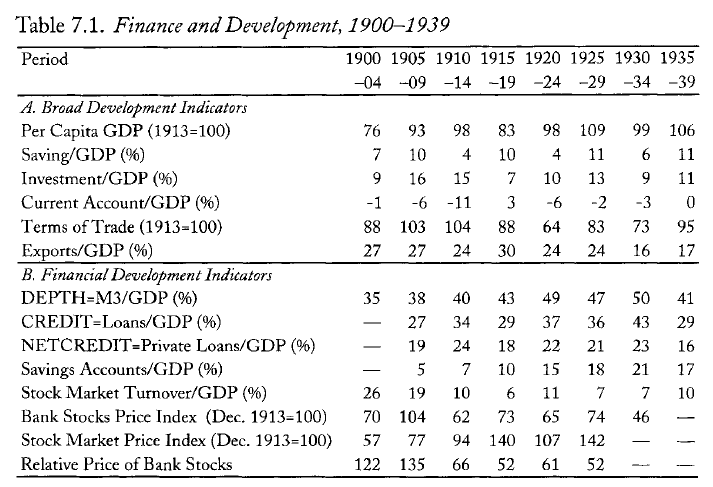
\includegraphics[scale=0.55]{uni2_dec20_02}
 
  \label{fig:uni1_01}
\end{figure} 
  \end{frame}


\begin{frame}\frametitle{Los años veinte, 1919-1928 (cont.)}
    \begin{itemize}\itemsep 10pt
      \item Puede verse que Argentina sufrió una fuerte desaceleración
        en el crecimiento luego de la 1GM --tasa de crecimiento en los
        20s de sólo 1.7\%
        \item Observe como en dos de los periodos de peor desempeño
          --1915/19 y 1930/34- la inversion es de las mas bajas del
          período (nunca logró recuperar el 15\% del PBI del periodo
          de oro)
          \item Igualmente puede verse la aumentada autarquía de la
            economía en este periodo --caida de CC/PBI (caida de
            CK/PBI) y caida en TDI
                   \end{itemize}
      \end{frame}


      \begin{frame}\frametitle{Los años veinte, 1919-1928 (cont.)}
    \begin{itemize}\itemsep 10pt
      \item Mirando a la parte financiera de la economia, puede
        observarse 2 (dos) indicadores tradicionales del desarrollo
        financiero: 1) $M3/GDP$ (``DEPTH'') y 2) $Préstamos/GDP$
        (``CREDIT'')
        \item Si bien DEPTH tiene una tendencia levemente ascendente
          durante el período (desde 35\% a 50\%), cuando uno mira
          CREDIT claramente se ven las debilidades
          \item El crédito total sube de 27\% a 40\% hasta 1930 pero
            el crédito neto ($PréstamosPrivados/GDP$) cayó durante la
            1GM, se recuperó en los 20s para caer luego en la GD
                   \end{itemize}
      \end{frame}


       \begin{frame}\frametitle{Los años veinte, 1919-1928 (cont.)}
    \begin{itemize}\itemsep 10pt
      \item Esto sugiere que a pesar de que la economía argentina
        presentó un grado significativo de \textbf{monetización} no
        repercutió en un mayor desarrollo financiero (medido por una
        expansión del crédito bancario)
        \item En otras palabras, la mayor monetización y crecimiento
          de los depósitos no se tradujo en un movimiento gradual y
          sostenido de mayor crédito privado a la inversión --en
          definitiva la mejor expresión del desarrollo financiero
                   \end{itemize}
      \end{frame}
      
      

   \begin{frame}\frametitle{Los años veinte, 1919-1928 (cont.)}
    \begin{itemize}\itemsep 10pt
      \item Estudios argumentan que mayor desarrollo financiero puede
        aumentar crecimiento hasta en 0.5\% promedio por año
        $\longrightarrow$ muy alejado de lo que ocurrio en Argentina
        \item Ante la ausencia de capital extranjero entre 1914 y
          1945, Argentina tuvo que financiar su inversión doméstica
          con ahorro doméstico $\longrightarrow$ el sistema financiero
          no pudo responder
          \item La consecuencia de esto (restricción de capital) fue
            el retraso económico $\longrightarrow$ sistema financiero
            falló en dos tareas: 1) movilizar \textit{mas} capital; 2)
            aumentar \textit{eficiencia} en asignación de capital
                   \end{itemize}
      \end{frame}



       \begin{frame}\frametitle{Los años veinte, 1919-1928 (cont.)}
    \begin{itemize}\itemsep 10pt
      \item Uno de los problemas del contexto internacional causado
        durante la 1GM fue la suspensión del patrón oro estricto en
        todos los países durante 1914-19.
        \item Tuvo un corto y dinámico \textit{revival} en el segundo
          lustro de los 20s --\textit{patrón oro lingote} sin
          acuñación [David Ricardo]
          \item Gran Bretaña vuelve al patrón en 1925, a fines de la
            década casi 50 países operaban nuevamente bajo patrón oro
                   \end{itemize}
      \end{frame}
      
      

 \begin{frame}\frametitle{El frente externo: 1919-1928}
    \begin{itemize}\itemsep 10pt
      \item La balanza de pagos tuvo un comportamiento diverso en este
        período --positiva entre 1919 y 1921, negativa entre 1921 y
        1924 y positiva desde 1925
        \item El movimiento más notable fue el de la cuenta capital
          --se revierte de negativa en 1919-21 a positiva en el resto
          de la década
          \item La balanza comercial por su parte se mantiene
            superavitaria aunque con saldos significativamente mas
            bajos que durante el periodo de la 1GM
                   \end{itemize}
      \end{frame}



      
 \begin{frame}\frametitle{El frente externo: 1919-1928 (cont.)}
    \begin{itemize}\itemsep 10pt
      \item Otro contraste con el período anterior es que en la decada
        de los 20s los precios de X/M se mantuvieron relativamente
        estables pero las cantidades exportadas subieron
        \item Salvo durante el período 1921-1924 (crisis internacional
          y deflación) 
          que hubo salida de
          reservas, en general durante esta década la performance de
          las cuentas externas argentinas fue similar en terminos de
          BP pero diferente en la composición --volvió a entrar K pero
          se redujo el superavit comercial  
                   \end{itemize}
      \end{frame}
      
      

       \begin{frame}\frametitle{La Caja de Conversión: 1919-1928}
    \begin{itemize}\itemsep 10pt
      \item El sistema de papel moneda incovertible con tipo de cambio
        flexible seguido desde 1914
        continuaría hasta 1927 $\longrightarrow$ continuó con la
        lógica de ``autoregulación''
\item Variaciones (+/-) de reservas no son seguidas por variaciones en
  BM --en el 82\% de los descensos y 75\% de aumentos de reservas, la BM no varió.
\item ¿Cómo afecta esto al tipo de cambio peso mn/peso oro?
  \begin{itemize} \itemsep 10pt \medskip
  \item Bajan reservas y BM constante $\longrigtharrow$
    depreciación
    \item Suben reservas y BM constante $\longrightarrow$ apreciación
    \end{itemize}
    \item Al haber sido la BP positiva en gran parte de estos años, en
      1927 Argentina tenía un TC igual al de 1902. 
      \end{itemize}
      \end{frame}

       \begin{frame}\frametitle{La Caja de Conversión: 1919-1928 (cont.)}
\begin{figure}[hxtbp]\vspace{0cm}
  \centering
  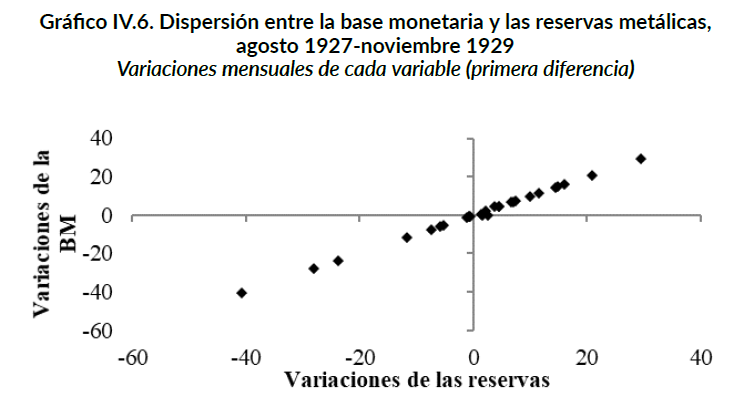
\includegraphics[scale=0.55]{uni2_dec20_05}
   \label{fig:uni1_01}
\end{figure} 
  \end{frame}
      


         \begin{frame}\frametitle{La Caja de Conversión: 1919-1928 (cont.)}
    \begin{itemize}\itemsep 10pt
      \item ¿Qué paso con el FDC? Luego de la movilizacion de los 20
        millones durante la 1GM, se utilizó el remanente de 10
        millones para pagar servicios de la deuda en 1924. Entre 1925
        y 1928 se volvió a integrar los 30 millones
                \item Note que en esta ocasión, sin embargo, el
                destino de los fondos del FDC fue el Estado --en otras
                palabras, se financió déficit acumulado
                      \end{itemize}
      \end{frame}


       \begin{frame}\frametitle{La Caja de Conversión: 1927-}
    \begin{itemize}\itemsep 10pt
    \item En 1927 se levanta la suspensión de la
      convertibilidad. Entre 1927 y 1929 la Argentina volvió un patrón
      oro de moneda convertible a la paridad de 2.27 $\longrightarrow$
      volvía también el \textbf{trilema macroeconómico}
      \item Como era de esperarse, los datos avalan que efectivamente
        Argentina se manejó en estos breves 28 meses siguiendo al
        principio de la \textbf{Currency School}.
        \item Hubo una estricta correlación entre los movimientos de
          las reservas y los movimientos de la BM
              \end{itemize}
      \end{frame}


       \begin{frame}\frametitle{La Caja de Conversión: 1927- (cont.)}
\begin{figure}[hxtbp]\vspace{0cm}
  \centering
  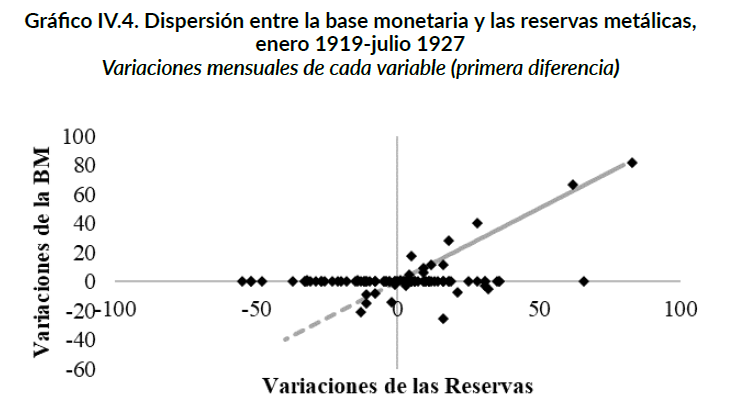
\includegraphics[scale=0.55]{uni2_dec20_06}
   \label{fig:uni1_01}
\end{figure} 
  \end{frame}
      


       \begin{frame}\frametitle{El sistema bancario}
    \begin{itemize}\itemsep 10pt
    \item El crecimiento de los depósitos bancarios en este período
      fue menor al necesario para volver a ubicarse en niveles de
      crecimiento previo a 1921
     \item Entre 1919 y 1928, la tasa de crecimiento de depositos (reales) fue de 6.9\%
       (BNA) y 6.0\% para el resto
       \item Mientras tanto, el ratio de reservas era del 27\% (BNA) y
         de 29\% para el resto. Puede notarse un decaimiento respecto
         de 1914-18. 
              \end{itemize}
      \end{frame}
      


   \begin{frame}\frametitle{Las cuentas públicas}
    \begin{itemize}\itemsep 10pt
    \item Luego de un equilibrio en el año 1920, las cuentas fiscales
      se deterioraron en el resto de la década --el resultado
      financiero fue siempre negativo mientras que el resultado
      primario fue positivo de 1923 a 1926
      \item Lo más importante sin embargo refiere a un aumento de la
        participación estatal en la economía --
              \end{itemize}
      \end{frame}
      
      


  \begin{frame}\frametitle{Las cuentas públicas (cont.)}
\begin{figure}[hxtbp]\vspace{0cm}
  \centering
  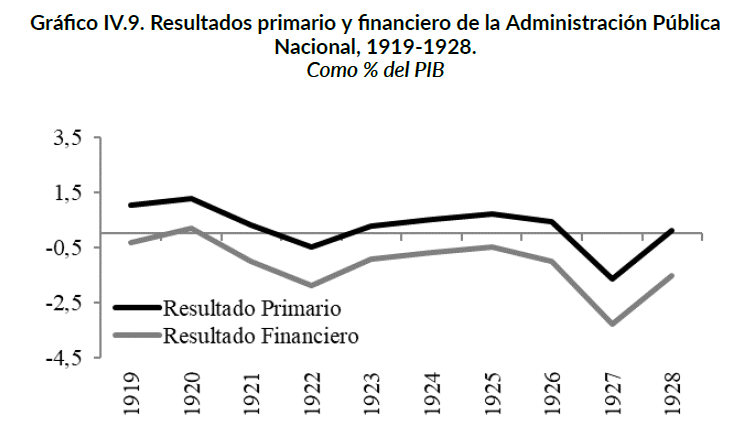
\includegraphics[scale=0.55]{uni2_dec20_03}
   \label{fig:uni1_01}
\end{figure} 
  \end{frame}
      



  \begin{frame}\frametitle{Las cuentas públicas (cont.)}
\begin{figure}[hxtbp]\vspace{0cm}
  \centering
  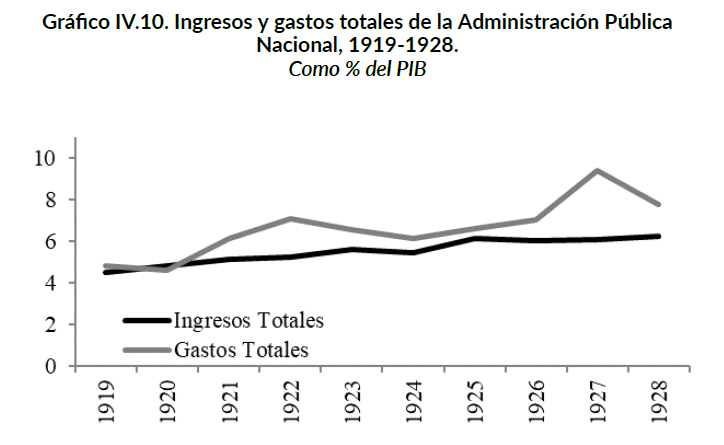
\includegraphics[scale=0.55]{uni2_dec20_04}
   \label{fig:uni1_01}
\end{figure} 
  \end{frame}
      


     \begin{frame}\frametitle{El BNA y las funciones banco-centralistas}
    \begin{itemize}\itemsep 10pt
    \item En este período es a partir de 1923 cuando el BNA empieza a
      usar fuertemente los redescuentos para sostener el sistema
      bancario/financiero --entre 1923 y 1928 el monto de redescuentos
      representó entre un 15\% y un 30\% de las reservas de los bancos
      \item Esto importa una fuerte contraste con el periodo de la 1GM
        en que solo fueron importantes en 1914
        \item De no haber existido redescuentos, el ratio de reservas
          a depósitos hubiera sido aún menor que el marcado anteriormente
              \end{itemize}
      \end{frame}
      


  \begin{frame}\frametitle{El BNA y las fuciones banco-centralistas (cont.)}
\begin{figure}[hxtbp]\vspace{0cm}
  \centering
  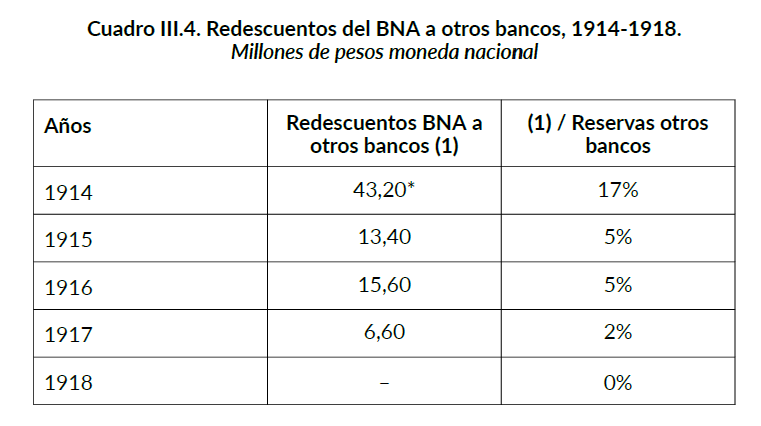
\includegraphics[scale=0.55]{uni2_dec20_07}
   \label{fig:uni1_01}
\end{figure} 
  \end{frame}
      

  
  \begin{frame}\frametitle{El BNA y las funciones banco-centralistas (cont.)}
\begin{figure}[hxtbp]\vspace{0cm}
  \centering
  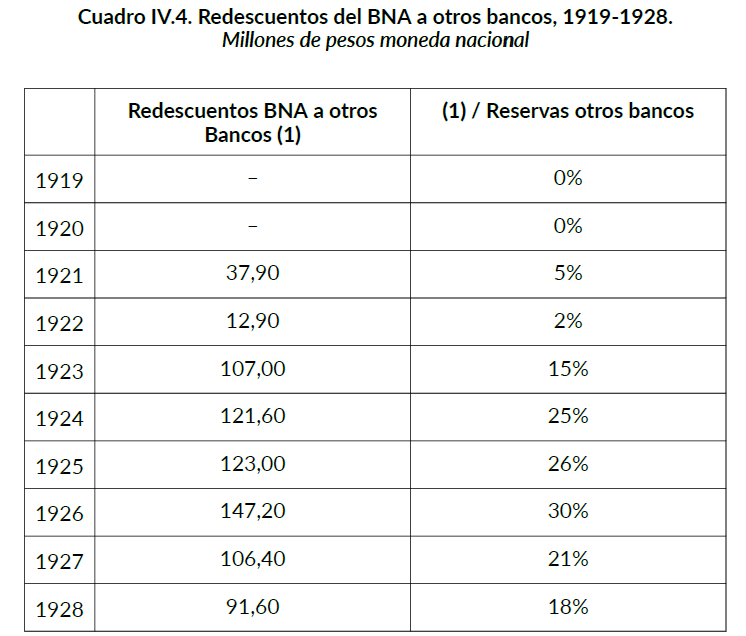
\includegraphics[scale=0.45]{uni2_dec20_08}
   \label{fig:uni1_01}
\end{figure} 
  \end{frame}
      
      
 \begin{frame}\frametitle{El BNA y el financiamiento al Estado}
    \begin{itemize}\itemsep 10pt
    \item El BNA siguió siendo la principal fuente de financiamiento
      del Estado incluso luego de haber finalizado la 1GM. Hubo saldos
      deudores en exceso del limite legal en los primeros años. El
      redescuento de Letras de Tesorería creció en forma importante
      \item Tambien crecieron los préstamos oficiales aunque en menor
        medida luego de 1925. Y los fondos públicos se mantuvieron
        alrededor de 40 millones
        \item Lo importante es que aparecieron nuevas fuentes y formas
          (partidas) de financiamiento del BNA al Estado
              \end{itemize}
      \end{frame}
      

  \begin{frame}\frametitle{El BNA y el financiamiento al Estado (cont.)}
\begin{figure}[hxtbp]\vspace{0cm}
  \centering
  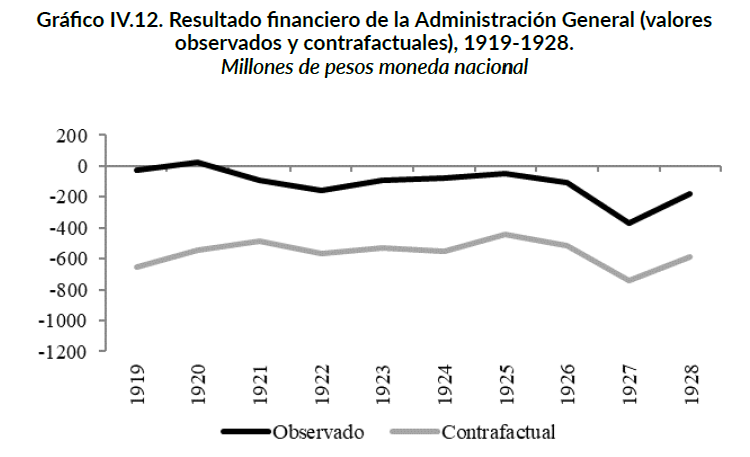
\includegraphics[scale=0.55]{uni2_dec20_09}
   \label{fig:uni1_01}
\end{figure} 
  \end{frame}
      
     
            
 \begin{frame}\frametitle{El BNA y el financiamiento al Estado (cont.)}
    \begin{itemize}\itemsep 10pt
    \item ¿Cómo afectó esto al BNA y su posición de liquidez? La
      respuesta es que el financiamiento que el BNA realizó al Estado
      nacional le impidió continuar con una muy fuerte y sólida
      posición de reservas (a diferencia del que realizó a sistema
      bancario)
      \item Si no hubiera financiado al Estado, su nivel de reservas
        hubiera sido 30 puntos mas; si no hubiera financiado al
        sistema bancario, hubiera sido solo 6 puntos mas. 
              \end{itemize}
      \end{frame}
      


        \begin{frame}\frametitle{El BNA y el financiamiento al Estado (cont.)}
\begin{figure}[hxtbp]\vspace{0cm}
  \centering
  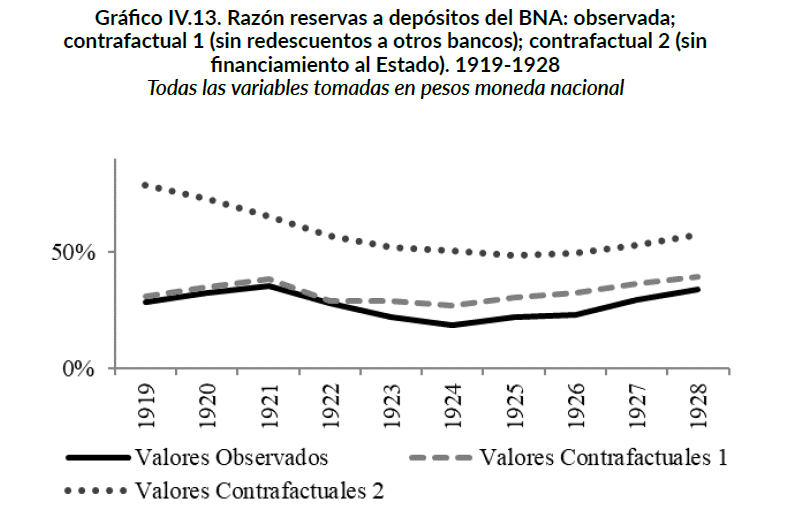
\includegraphics[scale=0.55]{uni2_dec20_10}
   \label{fig:uni1_01}
\end{figure} 
  \end{frame}
      


      
      
\end{document}

      